\documentclass[t]{beamer}
\usetheme[deutsch]{KIT}
\setbeamercovered{transparent}
\setbeamertemplate{navigation symbols}{}

\KITfoot{Tutoriumsmaterial von Alexander Kwiatkowski, Michael Vollmer und Matthias Holoch \hspace{2.5cm} Basierend auf den Folien von Simon Stroh und Moritz v. Looz}
\usepackage[utf8]{inputenc}
\usepackage{amsmath}
\usepackage{ifthen}
\usepackage{amssymb}
\usepackage{tikz}
\usepackage{ngerman}
\usepackage[normalem]{ulem}
\usetikzlibrary{automata}
\usenavigationsymbols


\title{Theoretische Grundlagen der Informatik}
\subtitle{Tutorium}
\author{Alexander Kwiatkowski, Michael Vollmer und Matthias Holoch}

\institute[IKS]{Institut für Kryptographie und Sicherheit}

\TitleImage[height=\titleimageht]{images/tmaschine.png}

\newcommand{\N}{\ensuremath{\mathbb{N}}}
\newcommand{\M}{\ensuremath{\mathcal{M}}}
\newcommand{\classP}{\ensuremath{\mathcal{P}}}
\newcommand{\classNP}{\ensuremath{\mathcal{NP}}}
\newcommand{\co}{\ensuremath{\mathsf{co\text{-}}}}
\newcommand{\pot}{\ensuremath{\mathcal{P}}}
\newcommand{\abs}[1]{\ensuremath{\left\vert #1 \right\vert}}
\newcommand{\menge}[2]{\ensuremath{\left\lbrace #1 \,\middle\vert\, #2 \right\rbrace}}
\newcommand{\ducttape}[1]{\vspace{#1}}
\newcommand{\neglit}[1]{\overline{#1\vphantom{x^a}}}
\newcommand{\recipe}{\raisebox{-.3cm}{
\includegraphics[scale=.15]{images/chefs-cap.png}}\hspace{0.2cm}}
\newcommand{\opt}[1]{\ensuremath{\text{OPT}(#1)}}
\newcommand{\A}[1]{\ensuremath{\mathcal{A}(#1)}}
\renewcommand{\O}[1]{\ensuremath{\mathcal{O}(#1)}}
\newcommand{\msout}[1]{\text{\sout{\ensuremath{#1}}}}

\newcommand{\invincible}{\setbeamercovered{invisible}} %  "Yesss! I am invincible!!" (Boris Grishenko)
\newcommand{\vincible}{\setbeamercovered{transparent}}
\renewcommand{\solution}[1]{\invincible \pause #1 \vincible}
\newcommand{\micropause}{\\[8pt]}

% \@ifundefined{tikzset}{}{\tikzset{initial text=}} % Text "start" bei Startknoten unterdrücken
\tikzstyle{every node}=[thick]
\tikzstyle{every line}=[thick]

\newcommand{\tutnr}[1]{
  \subtitle{Tutorium #1}
	\begin{frame}
		\maketitle
	\end{frame}
}

\newcommand{\uebnr}[1]{
  \subtitle{Anmerkungen zum #1. Übungsblatt}
	\begin{frame}
		\maketitle
	\end{frame}
}

\begin{document}

\uebnr{4}

\invincible

\begin{frame}
	\frametitle{Komplexitätsfragen}
	
	Ist folgende Sprache über $\Sigma = \{a, \ldots, z\}$ in \classP{}? $$L := \menge{\left\langle x, k \right\rangle}{x \in \Sigma^*, \text{ in } x \text{ kommt mindestens } k \text{-mal das Zeichen } a \text { vor} }$$
	
	\pause Ich behaupte: \textbf{Nein,} wenn $\classP \neq \classNP$!
	
	\pause Begründung: $L$ ist das CLIQUE-Problem, und CLIQUE ist \classNP{}-vollständig.
	
	\pause
	\begin{itemize}
		\item Knoten $\mathop{\hat{=}}$ Zeichen von $x$
		\item Kanten: zwischen $a$-Knoten
		\item Cliquengröße: $k$
	\end{itemize}
	
	\pause Beispiel: $x = panamakanal$, $k = 5$ $\Rightarrow$
	
	\raggedleft { \ducttape{-2.5cm} 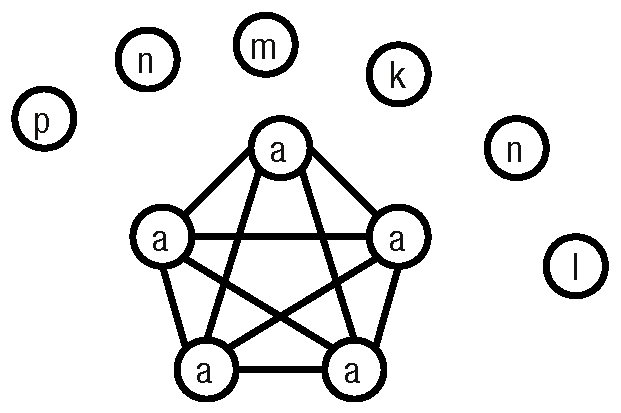
\includegraphics[scale=.6]{images/panama.pdf} }
	
\end{frame}

\begin{frame}
	\frametitle{Quatsch mit Soße!}
	
	\begin{itemize}
	\item	Ich habe gerade gezeigt: $L$ $\propto$ CLIQUE.
	\item In Worten: CLIQUE ist mindestens so schwer wie $L$.
	\item Irgendwie klar, da CLIQUE $\classNP$-vollständig, also $\classNP$-schwer.
	\item Für die $\classNP$-Vollständigkeit von $L$ wäre aber zu zeigen: CLIQUE	$\propto$ $L$.
	\end{itemize} 
	
	\pause
	
	\begin{block}{Merke:}
	\alert{Um zu zeigen, dass ein Problem \textit{nicht} in \classP{} liegt, muss man ein anderes Problem, das nicht in \classP{} liegt, \textbf{auf dieses Problem reduzieren}!}
	\end{block}
\end{frame}

\vincible

\begin{frame}
	\frametitle{Allgemeines}
	
	\begin{itemize}
		\item Beschreibungen in Beweisen: oft \textit{sehr} schwammig
		\begin{itemize}
			\item In der Klausur wird vermutlich strenger korrigiert!
		\end{itemize}
		\pause \item Optimierungsproblem $\rightarrow$ Entscheidungsproblem:
		\begin{itemize}
			\item Optimierungsproblem: "`Finde eine optimale Lösung"' \\ Entscheidungsproblem "`Existiert eine Lösung mit Wert $k$?"'
		\end{itemize}
		\pause \item Semientscheidbare Sprachen
		\begin{itemize}
			\item Sei $L$ eine semientscheidbare Sprache, die von einer TM $\mathcal{M}$ erkannt wird.
			\item Was macht $\mathcal{M}$ für eine Eingabe $x \in L$?
			\pause \item Was macht $\mathcal{M}$ für eine Eingabe $x \not\in L$?
		\end{itemize}
	\end{itemize}
\end{frame}

\frame{
  \frametitle{Lizenzen}
  \center
  
\includegraphics[width=2em]{images/by}
  
\includegraphics[width=2em]{images/cc}
  
\includegraphics[width=2em]{images/sa}
  \\
  {\tiny

Dieses Werk ist unter einem ``Creative Commons Namensnennung-Weitergabe unter gleichen Bedingungen 3.0 Deutschland``-Lizenzvertrag lizenziert. Um eine Kopie der Lizenz zu erhalten, gehen Sie bitte zu \href{http://creativecommons.org/licenses/by-sa/3.0/de/}{http://creativecommons.org/licenses/by-sa/3.0/de/} oder schreiben Sie an Creative Commons, 171 Second Street, Suite 300, San Francisco, California 94105, USA.\\
  \vspace{1cm}
  Davon ausgenommen sind das Titelbild, welches aus der März-April 2002 Ausgabe von American Scientist erschienen ist und ohne Erlaubnis verwendet wird, sowie das KIT Beamer Theme. Hierfür gelten die Bestimmungen der jeweiligen Urheber.
  \vspace{1cm}
  \\ 
  }
  %Habe hier die Reihenfolge etwas umgestellt, weil die Formatierung bei mir komisch aussah. 
  %Wenn es bei dir anders ist, kannst du es auch wieder zurückändern, dann haben wir unterschiedliche Kompilieroptionen
}

\end{document}
